\label{sec:fak_sol}
In this section, we analyse the conformation of soluted FAK (FAK-SOL) in order to retrieve a reference state for later comparisons. Since the secondary structure of the two domains is fixed due to the elastic network, the focus is on the FERM-kinase interface.\\
\\
The first approach to describe the FERM-kinase interface is to consider the COM distances of F1 to the N-lobe ($d_\text{F1-N}$) and F2 to the C-lobe ($d_\text{F2-C}$).\\
The two dimensional histogram of these distances reveals two different states (see \autoref{free:f2clf1nl}). Spot 1 refers to conformations, which are partially opened at the F2 - C-lobe interface, but close at the F1 - N-lobe interface. In contrast to this, the conformations of spot 2 refers to states in which F2 and the C-lobe gets closer while the distance between F1 and the N-lobe is increased. The corresponding 3D structures are shown in \autoref{free:3d}. They imply that spot 1 refers to a configuration in which the kinase is slightly tilted against the FERM domain while it is in line for configurations associated with spot 2.\\
We observed several transitions between the spots during the simulation, which indicates a sufficiently long simulation time. In total $47.4\%$ of the obtained distances were located in spot 1 and $52.6\%$ in spot 2.\\
\\
A second important quantity associated to the FERM-kinase interface is the contact area (CA) of the interface. However, the observed two state system can not be identified in the CA values (see \autoref{free:ca}), since spot 2 shows only a slightly larger mean value of $27.6\,\si{\nano\metre}^2$ as compared to $27.1\,\si{\nano\metre}^2$ in spot 1.\\
%
%
%
\begin{figure}
	\subcaptionbox{\label{free:f2clf1nl}}[0.49\textwidth]{
		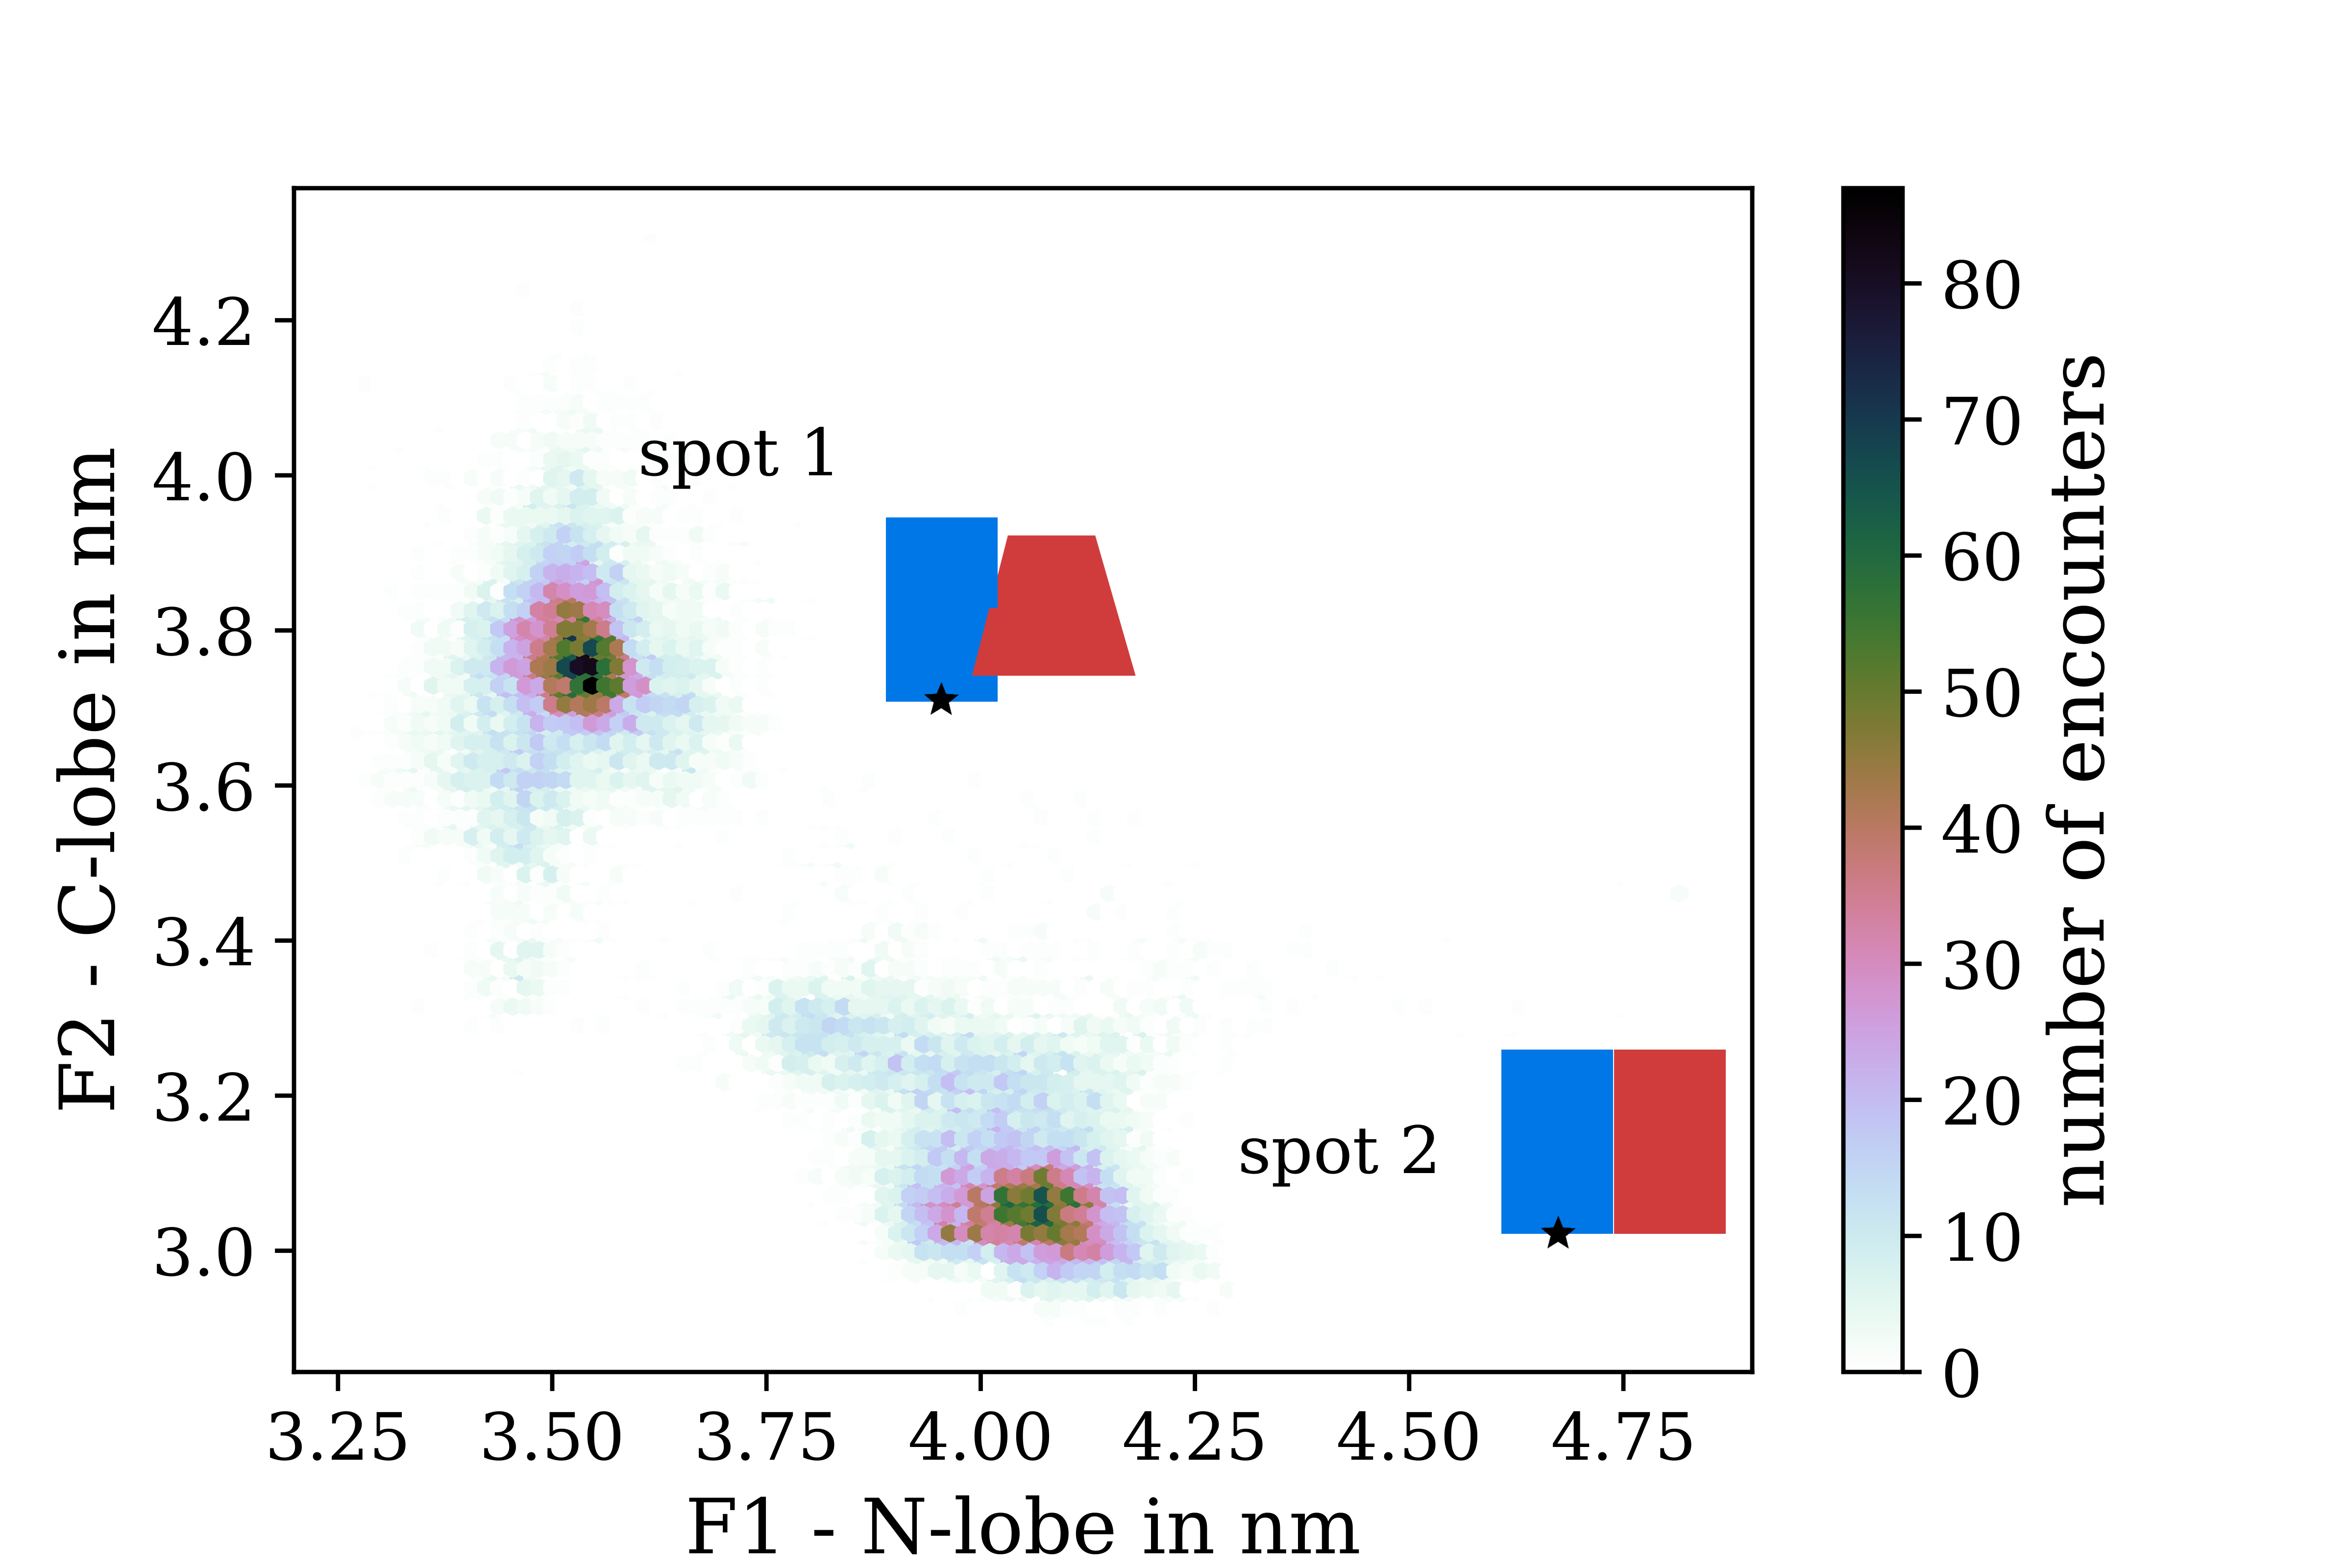
\includegraphics[height=5.2cm]{figures/results/free_f1f2_withcartoons}
	}\hfill%
	\subcaptionbox{\label{free:ca}}[0.49\textwidth]{
		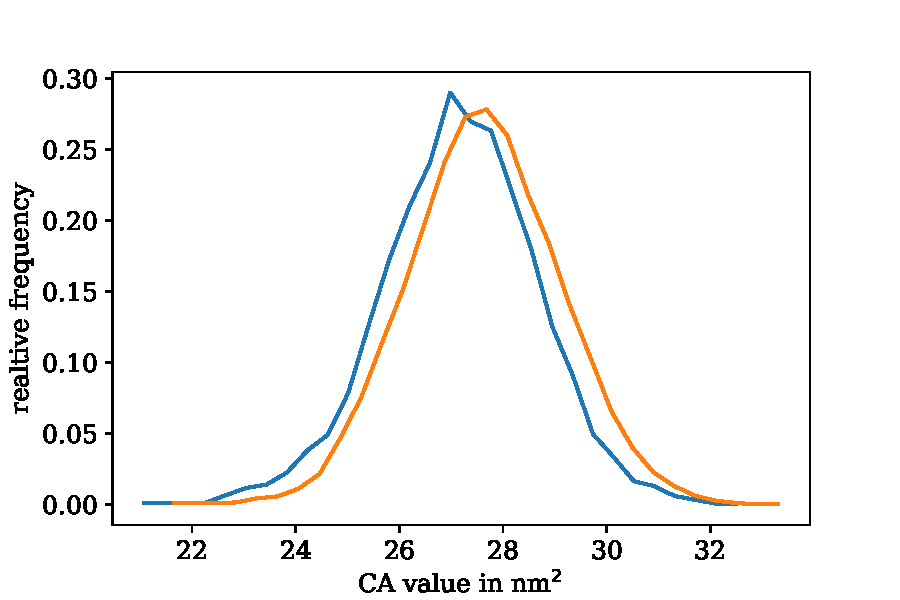
\includegraphics[height=5.2cm]{figures/results/free_ca}
	}%
	\nicecaption{Domain distances and contact area of FAK-SOL}{(\subref{free:f2clf1nl}): two dimensional hexagonal binning plot of $d_\text{F1-N}$ and $d_\text{F2-C}$ which implies a two state system. The tilting of the kinase (red) against the FERM domain (blue) is sketched beside. (\subref{free:ca}): Distribution of the CA value for the two obtained spots. The mean differs ca. $2\%$.}
	\label{free:pic_ca_and_com}
\end{figure}
%
%
%
\\
Finally, the contact map showing inter-residue distances of the FERM-kinase interface is considered. Both contact maps, for frames of spot 1 and frames of spot 2, show similar features. Hence, we only refer to the contact map of spot 2 in the following. However, contacts in area 2 are only observable in frames of spot 2 because the kinase is tilted against the FERM domain, \\
The average contact map for frames in spot 2 is shown in \autoref{free:contact}. Two regions can be identified. The first one (area 1) is located between F1 and the N-lobe/activation loop. It shows especially contacts between \acid{Y}{576} and \acid{Y}{577} and residues of the FERM domain. The minimal distance in this area, occurring between residue \acid{H}{41} and \acid{Y}{576}, is $0.45\,\si{\nano\metre}$ with an RMSF value of $0.03\,\si{\nano\metre}$. This area reflects the burying of the activity-regulating residues in the closed state (see \autoref{free:3d_spot2}).\\
The second region (area 2, obtained in spot 2 only) is located between F2 and the C-lobe. The spots occur around the residues \acid{Y}{180} and \acid{D}{200} of F2 as well as \acid{F}{596} and \acid{R}{665} of the C-lobe. The minimal distance in this area occurs between \acid{Y}{180} and \acid{F}{596} with $0.45\,\si{\nano\metre}$ and an RMSF value of $0.02\,\si{\nano\metre}$. Mutation experiments showed these two residues to have an important effect upon the interface \autocite{structFAK}, which fits to these observations.\\
The linker shows contacts with both domains. The minimal distances in the marked areas occur between the autophosphorylation site \acid{Y}{397} and \acid{H}{58} of F1 ($0.45\,\si{\nano\metre}$, RMSF $0.03\,\si{\nano\metre}$) as well as \acid{Y}{397} and \acid{Y}{576} of the kinase ($0.50\,\si{\nano\metre}$, RMSF $0.10\,\si{\nano\metre}$). Furthermore, several interactions occur between the residues in the linker itself, namely, between \acid{S}{379} to \acid{V}{389} and \acid{T}{394} to \acid{I}{400} (area 5). Also in this spot, the minimal distance occurs between \acid{Y}{397} and \acid{T}{386} ($0.52\,\si{\nano\metre}$, RMSF $0.04\,\si{\nano\metre}$). The density in this area implies that the linker forms a ball, which is slightly plunged into the interface of the FERM domain and the kinase (regarding area 3 and area 4). This can be seen also in the 3D structure in \autoref{free:3d_spot2}. Our observations support the thesis that autophosphorylation is prevented in the closed conformation by a binding of the linker to the FERM domain \autocite{pap003}.\\
%
%
\begin{figure}
	\centering
	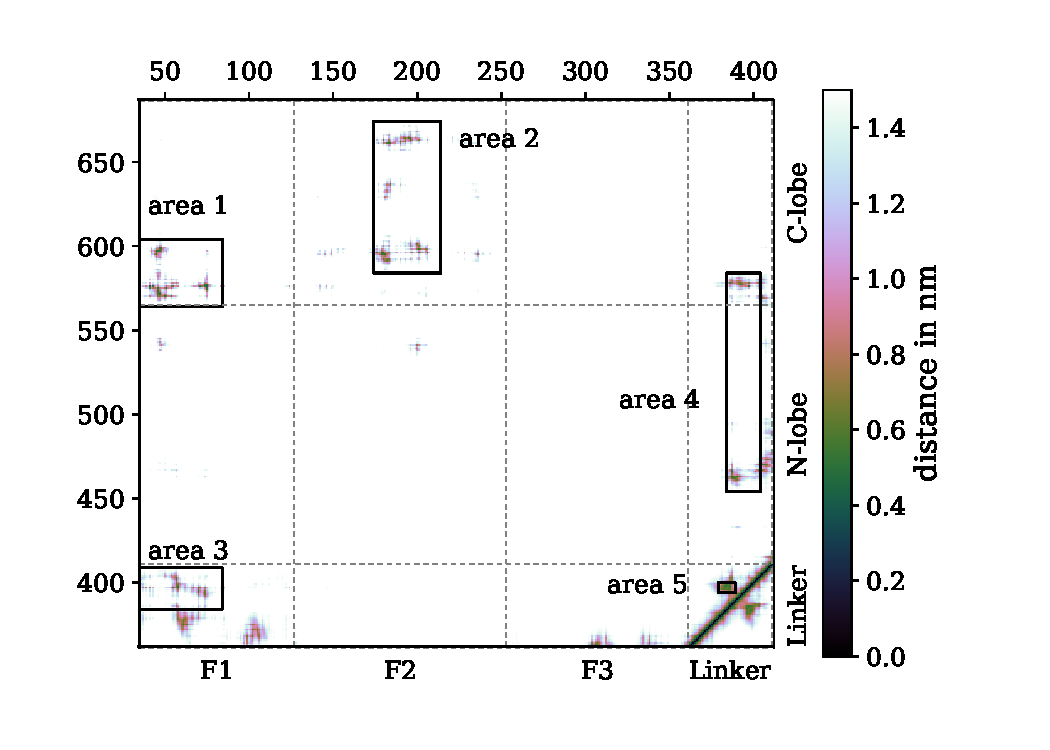
\includegraphics[width=.8\textwidth]{figures/results/contactmap_free}
	\nicecaption{Contact map of FAK-SOL}{Average contact map of the FERM-kinase interface and the linker region for frames of spot 2. The contact map for frames of spot 1 is similar, but lacks the contacts in area 2. In the contact map the burying of the active site (area 1) as well as the hiding of the autophosphorylation site \acid{Y}{397} (area 3, 4 and 5) can be seen.}
	\label{free:contact}
\end{figure}
%
%
%
%
%
%
\begin{figure}
	\subcaptionbox{\label{free:3d_spot1}}[0.32\textwidth]{
		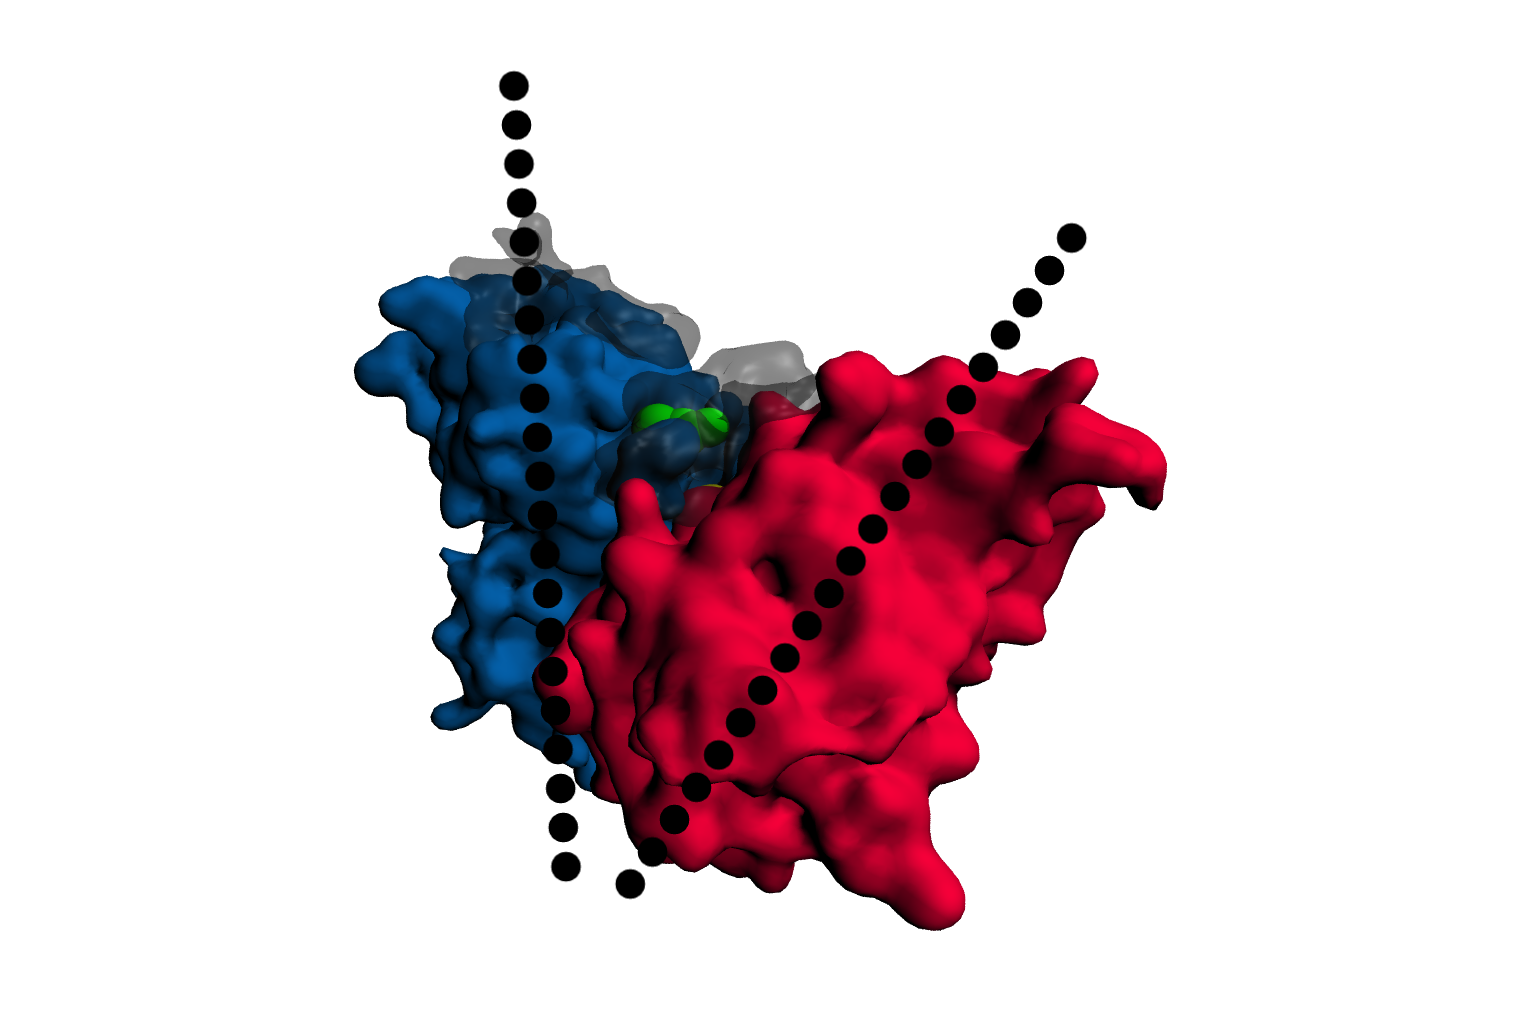
\includegraphics[height=4cm]{figures/results/fak_spot1}
	}\hfill%
	\subcaptionbox{\label{free:3d_spot2}}[0.32\textwidth]{
		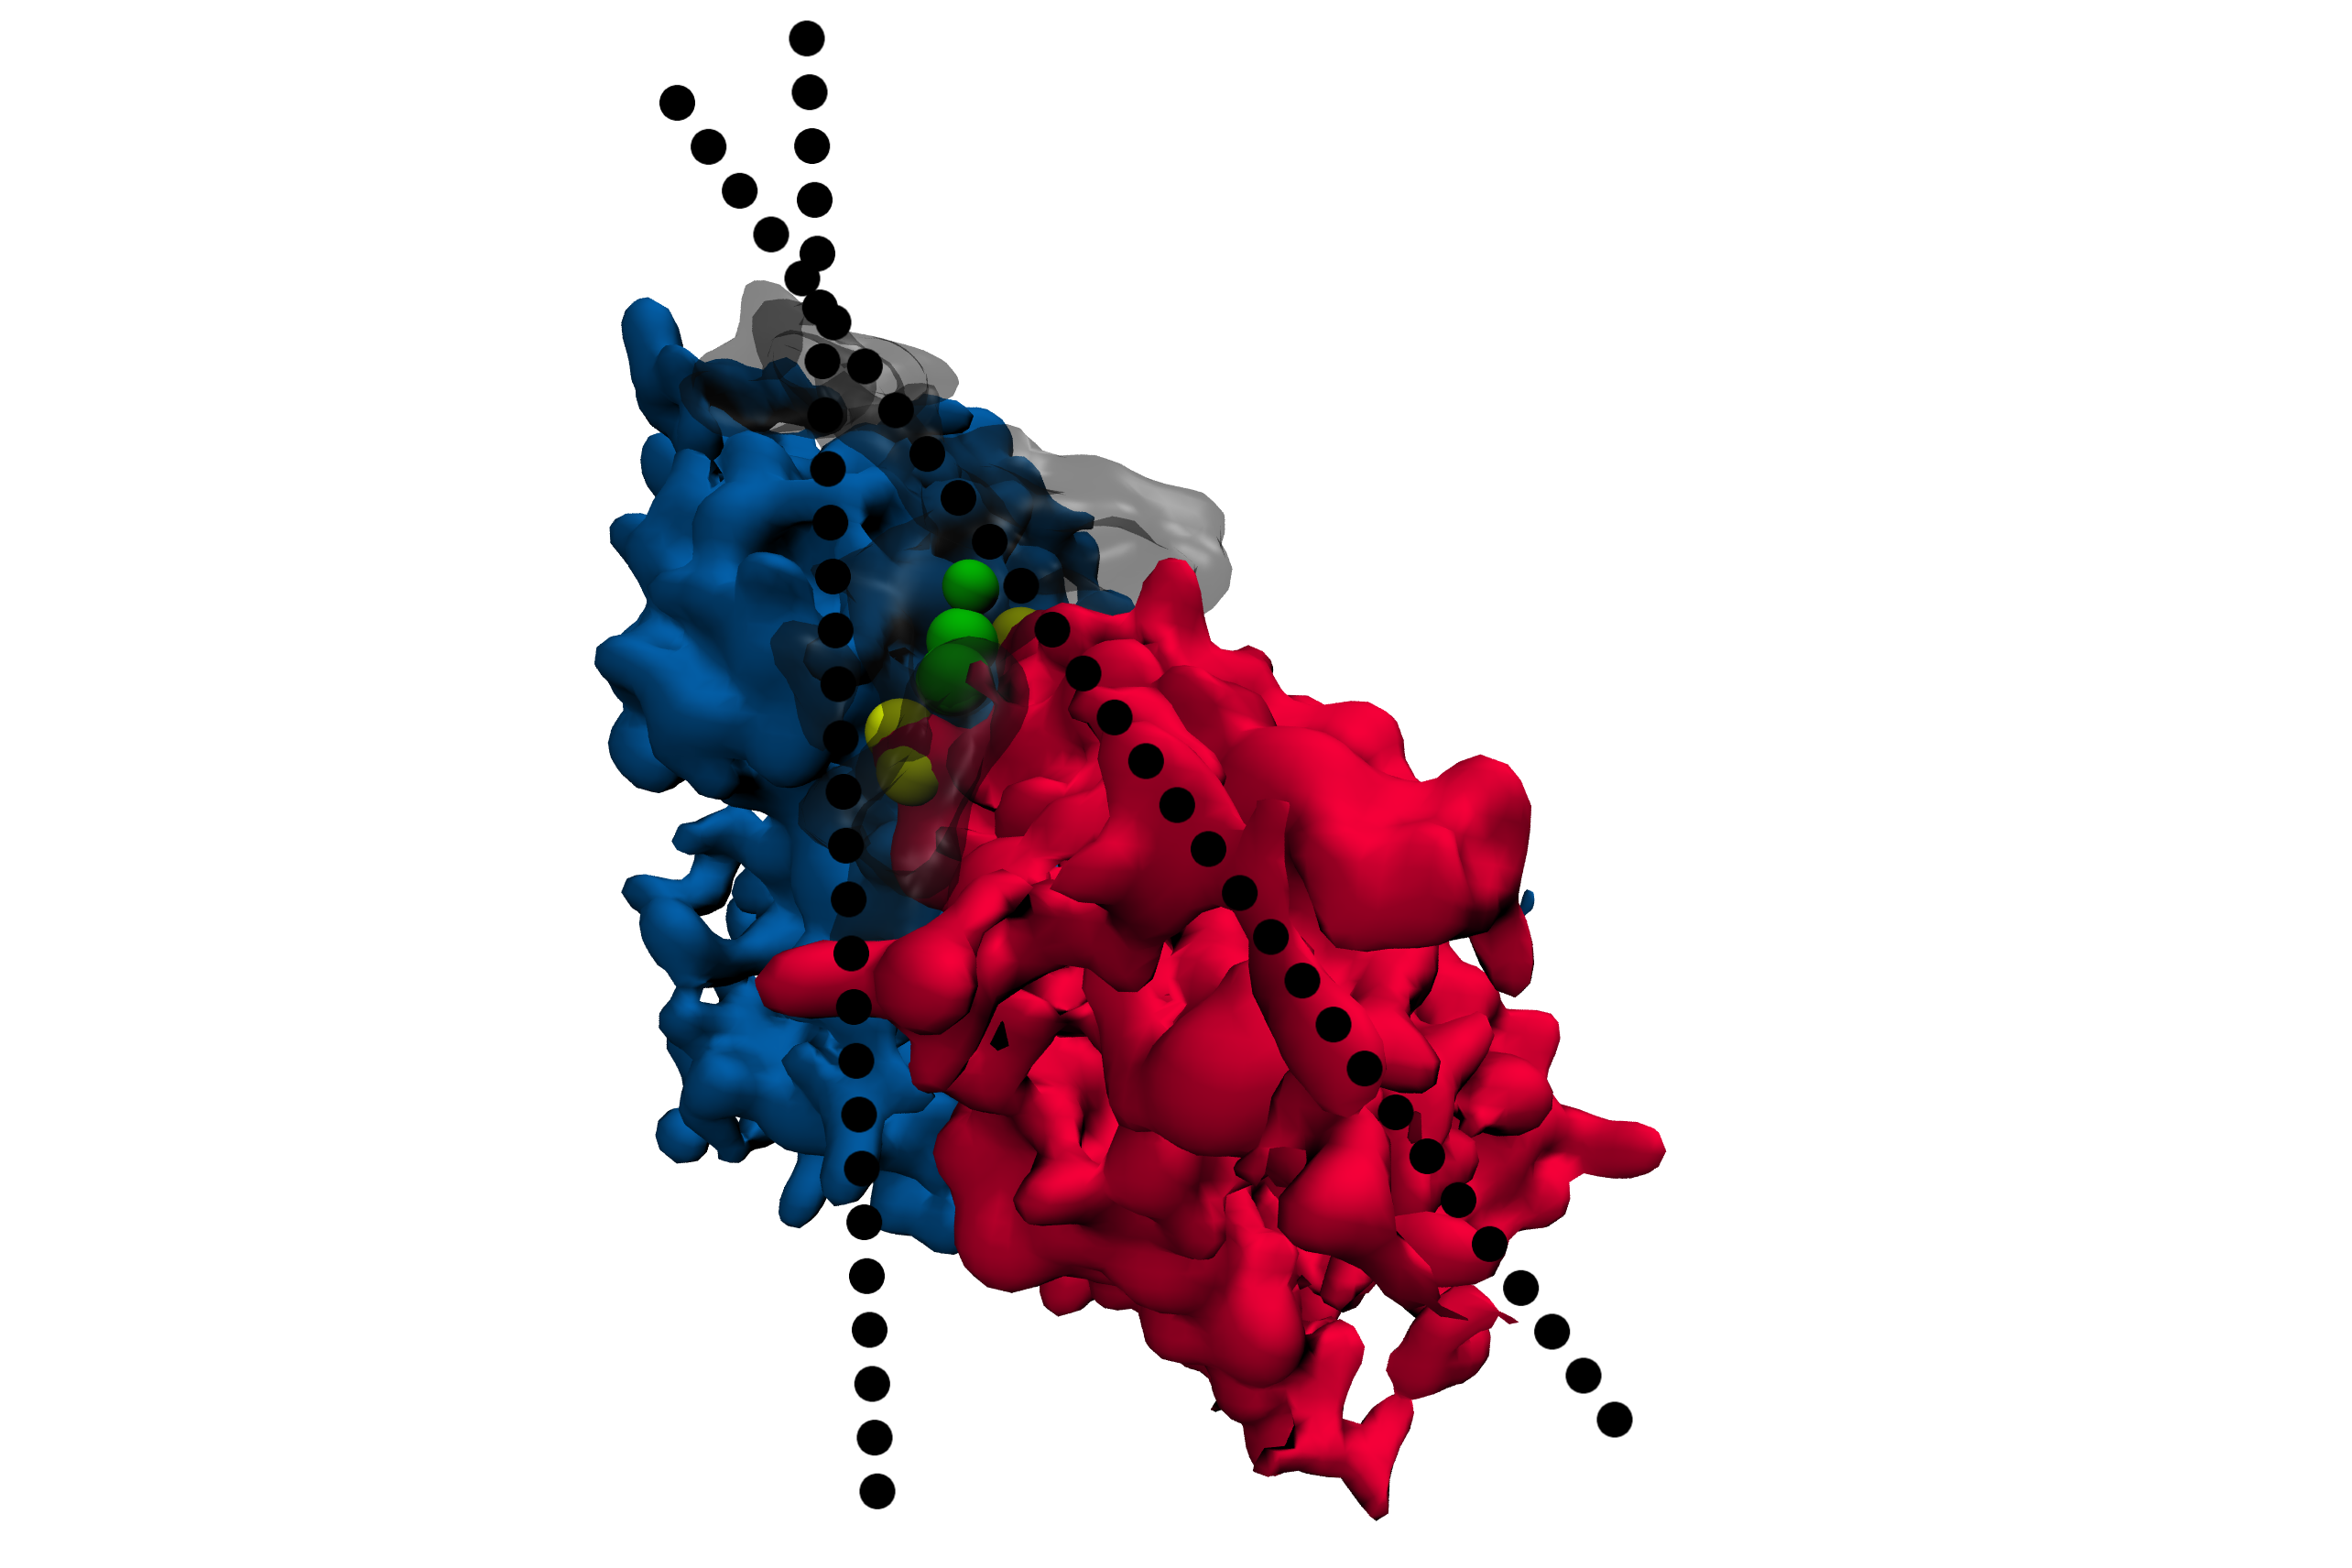
\includegraphics[height=3.5cm]{figures/results/fak_spot2}
	}\hfill%
	\subcaptionbox{\label{free:3d_spot_top}}[0.32\textwidth]{
		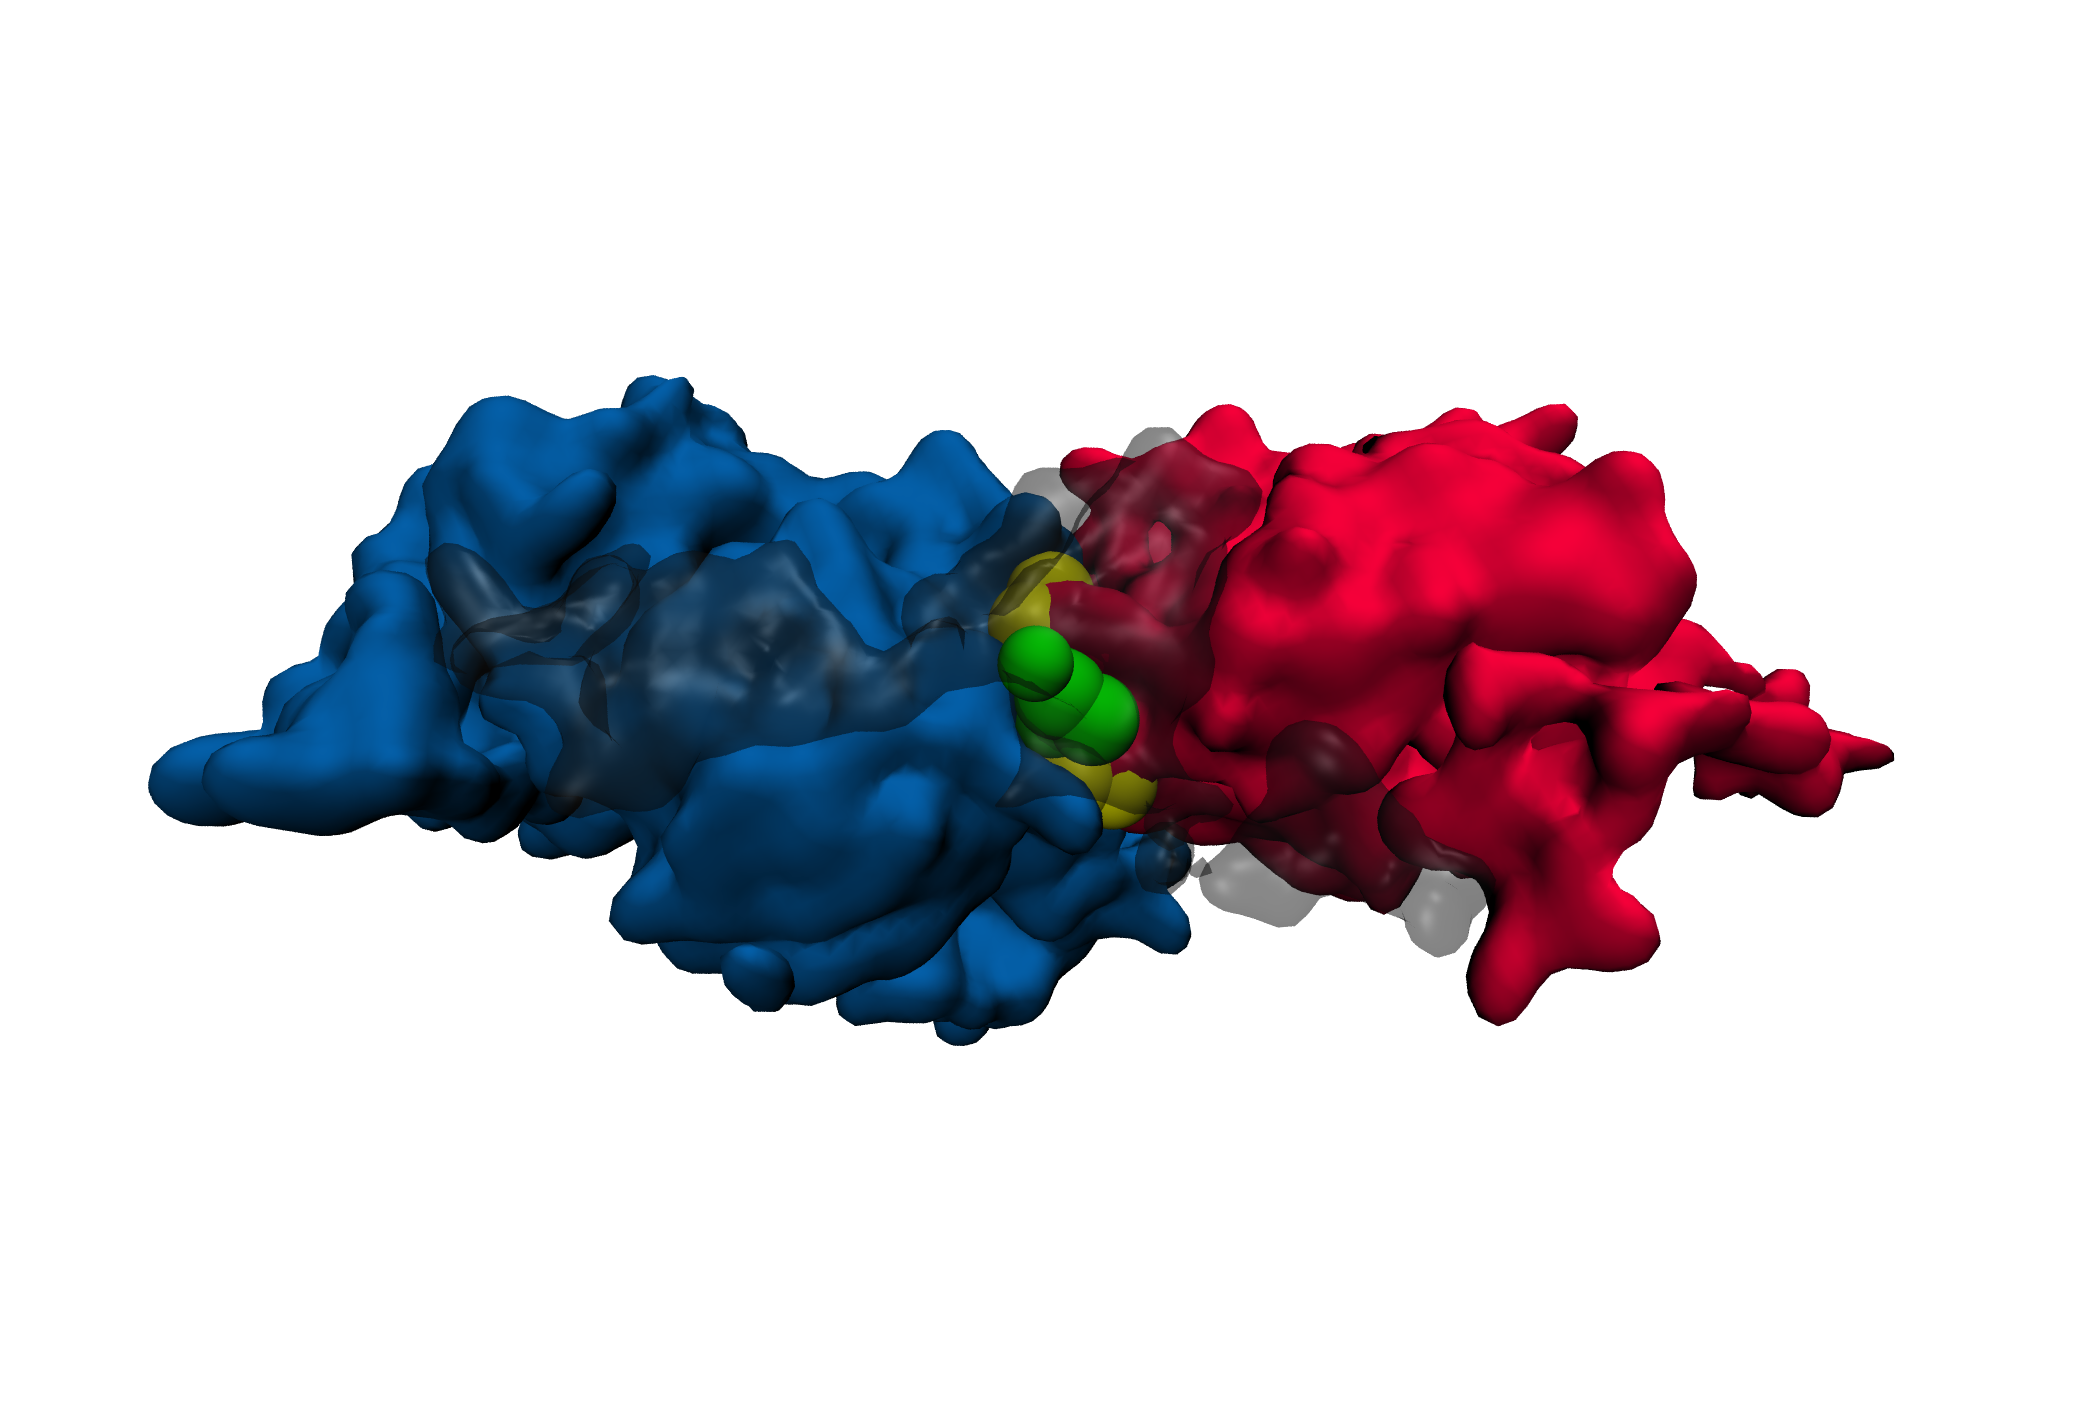
\includegraphics[height=3.5cm]{figures/results/fak_spot2_top}
	}
	\nicecaption{3D structure of the two states in FAK-SOL}{The 3D structures show the FERM domain (blue), the kinase (red) and the linker (black, transparent). The autophosphorylation site \acid{Y}{397} (green) is plunged into the interface and hidden by the linker. \acid{Y}{576} and \acid{Y}{577} (yellow) are shielded by the FERM domain.\\
	(\subref{free:3d_spot1}, spot 1): The kinase is tilted against FERM. (\subref{free:3d_spot2}, spot 2): Both domains are in line. (\subref{free:3d_spot_top}, spot 2): \acid{Y}{397}, \acid{Y}{576} and \acid{Y}{577} are shielded by the linker.}
\label{free:3d}
\end{figure}
%
%
%
